\begin{enumerate}
\item At a point $A$, $20$ metres above the level of water in a lake, the angle of elevation of a cloud is $30 \degree.$ The angle of depression of the reflection of the cloud in the lake, at $A$ is $60\degree .$ Find the distance of the cloud from $A$.
\item In Figure \ref{Figure 1}, a tower $AB$ is $20$ m high and $BC$, its shadow on the ground,is $20\sqrt{3}$ m long. Find the sun's altitude.
\begin{figure}[h!]
	\centering
    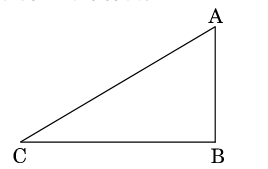
\includegraphics[width=0.5\columnwidth]{figs/cbse_30_3_1.png}
	\label{Figure 1}
\end{figure}
\item The angle of elevation of an aeroplane from a point $A$ on the ground is $60 \degree  $. After a flight of $15$ seconds, the angle of elevation changes to $  30 \degree.$ If the aeroplane is flying at a constant height of $1500\sqrt{3}$ m, find the speed of the plane in km/hr.
\end{enumerate}
